\documentclass[border=5pt]{standalone}
\usepackage{tikz}
\usepackage{amsmath}
\usetikzlibrary{calc}
\begin{document}
    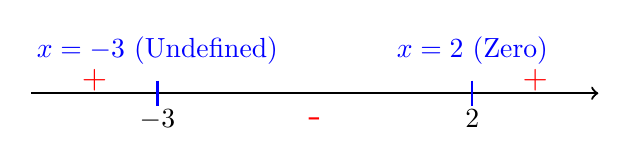
\begin{tikzpicture}[scale=0.8]
\draw[->, thick] (-5,0) -- (4,0); % 数轴从-5到4
\foreach \x in {-3,2}
\draw (\x,0.1) -- (\x,-0.1) node[below] {$\x$};
\node[above] at (-3,0.3) {\color{blue}$x=-3$ (Undefined)}; % 向上移动标签
\node[above] at (2,0.3) {\color{blue}$x=2$ (Zero)}; % 同样调整
\draw[blue, thick] (-3,0.2) -- (-3,-0.2);
\draw[blue, thick] (2,0.2) -- (2,-0.2);
\node[red] at (-4,0.2) {\large +}; % 在区间(-∞,-3)中间的位置
\node[red] at (-0.5,-0.4) {\Large -}; % 区间(-3,2)
\node[red] at (3,0.2) {\large +};
\end{tikzpicture}
\end{document}
